%-----------------------------------------------
% Dateiname: CreateTestsForOldAPI.tex
% Autor    : Stefano Kowalke <blueduck@gmx.net>
% Lizenz   : BSD
%-----------------------------------------------
\section{Implementation von Unit Tests der alten Datenbank API}
\label{prototype:sec:createTestForOldAPI}
Um zu gewährleisten, dass TYPO3 CMS sowohl mit der alten API - die von dem Prototypen zur Verfügung gesellt wird - als auch mit der neuen API kompatibel ist, müssen Untit Tests für die alte Datenbank API geschrieben werden. 

Zur Ausführung der Unit Tests wird die Extension \textit{PHPUnit} benötigt, welche das gleichnamige Testing Framework \textit{PHPUnit\footnote{\url{http://www.phpunit.de}}} zur Verfügung und einen einen graphischen Testrunner im Backend mitbringt. Sie wird über den Extension Manager installiert.

Die alte Datenbank API verfügt zur dem Zeitpunkt der Erstelltung des Prototypen über 40 Tests mit 49 Assertions, welche jedoch lediglich Hilfsmethoden testen. Im Laufe der Arbeit wurden wurden 68 Tests implementiert, die alle Methoden testen. Die Abbildung~\ref{fig:executeUnitTestsForOldAPI} zeigt die Ausführung der von TYPO3 CMS mitgelieferten Unit Tests; Abbildung~\ref{fig:executeNewUnitTestsForOldAPI} zeigt die Ausführung der neu implementierten sowie der alten Tests.

\begin{figure}[H]
    \centering
    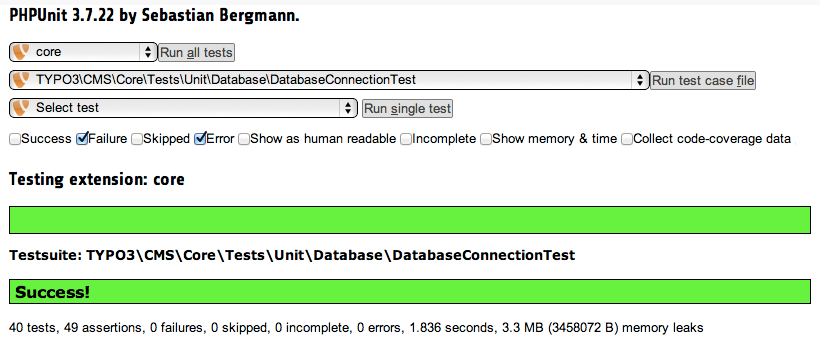
\includegraphics[scale=0.5]{TYPO3/DatabaseConnectionUnitTestsLegacy.png}
    \caption{Ausführung der vorhandenen Unit Tests für die alte Datenbank API}
    \label{fig:executeUnitTestsForOldAPI}
\end{figure}

\begin{figure}[H]
    \centering
    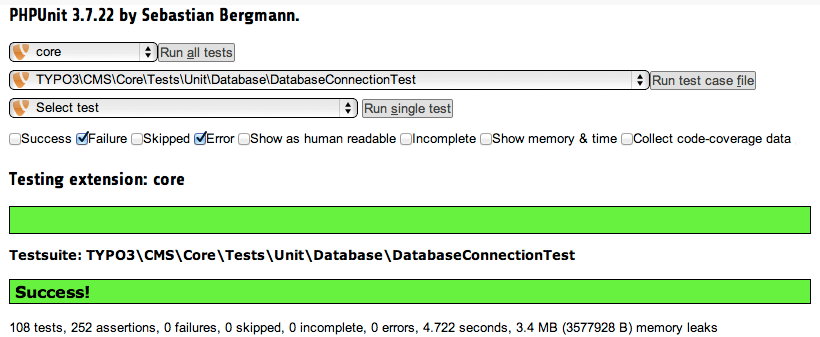
\includegraphics[scale=0.5]{TYPO3/DatabaseConnectionAddedUnitTestsLegacy.png}
    \caption{Ausführung der vorhandenen und hinzugefügten Unit Tests für die alte Datenbank API}
    \label{fig:executeNewUnitTestsForOldAPI}
\end{figure}
